\begin{figure}[t]
\centering
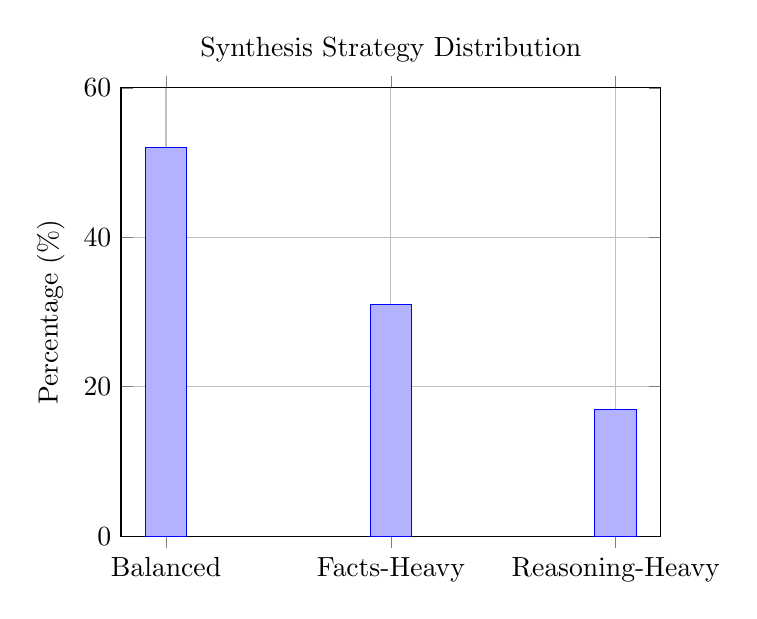
\begin{tikzpicture}
\begin{axis}[
    ybar,
    bar width=15pt,
    ylabel={Percentage (\%)},
    symbolic x coords={Balanced, Facts-Heavy, Reasoning-Heavy},
    xtick=data,
    ymin=0, ymax=60,
    legend pos=north east,
    grid=major,
    title={Synthesis Strategy Distribution}
]
\addplot coordinates {(Balanced,52) (Facts-Heavy,31) (Reasoning-Heavy,17)};
\end{axis}
\end{tikzpicture}
\caption{Distribution of synthesis strategy selection across 1,000 evaluated questions. The balanced strategy is most common (52\%), followed by facts-heavy (31\%) and reasoning-heavy (17\%), indicating that retrieval quality varies significantly across questions.}
\label{fig:agent_contribution}
\end{figure}
